\documentclass[12pt,a4paper,landscape]{article}
\usepackage{geometry}
\geometry{left=2.5cm,right=2.5cm,top=2.5cm,bottom=2.5cm}

\usepackage[utf8]{inputenc}
\usepackage{listings}
\usepackage{CJK}
\usepackage{xcolor}
\usepackage{graphicx}


\begin{document}
\begin{CJK}{UTF8}{gbsn}
\title{安装漂亮的Faenza1.3与Faience0.5图标主题}
\author{ismdeep}
\date{2013-4-22}


\maketitle

%设置listings
\lstset{numbers=left,
numberstyle=\tiny,
keywordstyle=\color{blue!100}, commentstyle=\color{red!50!green!50!blue!50},
frame=single,tabsize=4,showtabs=false,extendedchars=false,
rulesepcolor=\color{red!20!green!20!blue!20}
}


相信你不会认识这两款图标主题,非常漂亮的图标主题, Faenza 1.3 与 Faience 0.5 也一直在更新,而且也支持更多的应用图标。图标设计类似苹果的方块圆角,直观漂亮。两款主题的版本现在为 Faenza 1.3 与 Faience 0.5 。


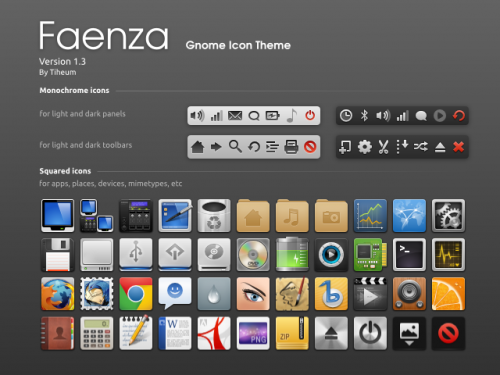
\includegraphics{2110193tcc350ztc2nkjxy.png}


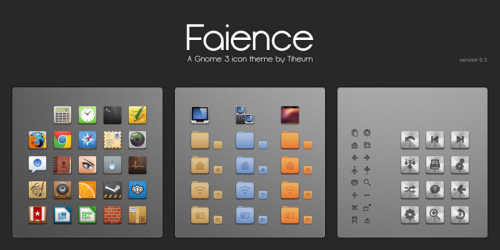
\includegraphics{211019va0xxz83s3xv6utz.png}


Ubuntu用户安装Faenza:

sudo add-apt-repository ppa:tiheum/equinox

sudo apt-get update

sudo apt-get install faenza-icon-theme

安装Faience:

sudo add-apt-repository ppa:tiheum/equinox

sudo apt-get update

sudo apt-get install faenza-icon-theme faience-icon-theme 






\end{CJK}
\end{document}


